\section{System Architecture}
\label{sec:architecture}

The techniques used to measure probabilistically bounded staleness (PBS) are
applicable to any system for which we can model the replication protocol used.
PBS predictions require some lightweight latency profiling in the underlying
datastore and we have implemented this profiling module in Cassandra and
Voldemort, two widely used distributed key-value stores. In this section, we
describe our experience in implementing and integrating PBS in these data
stores. We also explain some of the design decisions we made to simplify the
integration and how this could be generalized to other systems. 

%Introductory paragraph explaining the system architecture. Explain that our
%approach is to make PBS a shim layer on top of existing server code. Latency
%measurements etc.

\begin{figure}
\centering
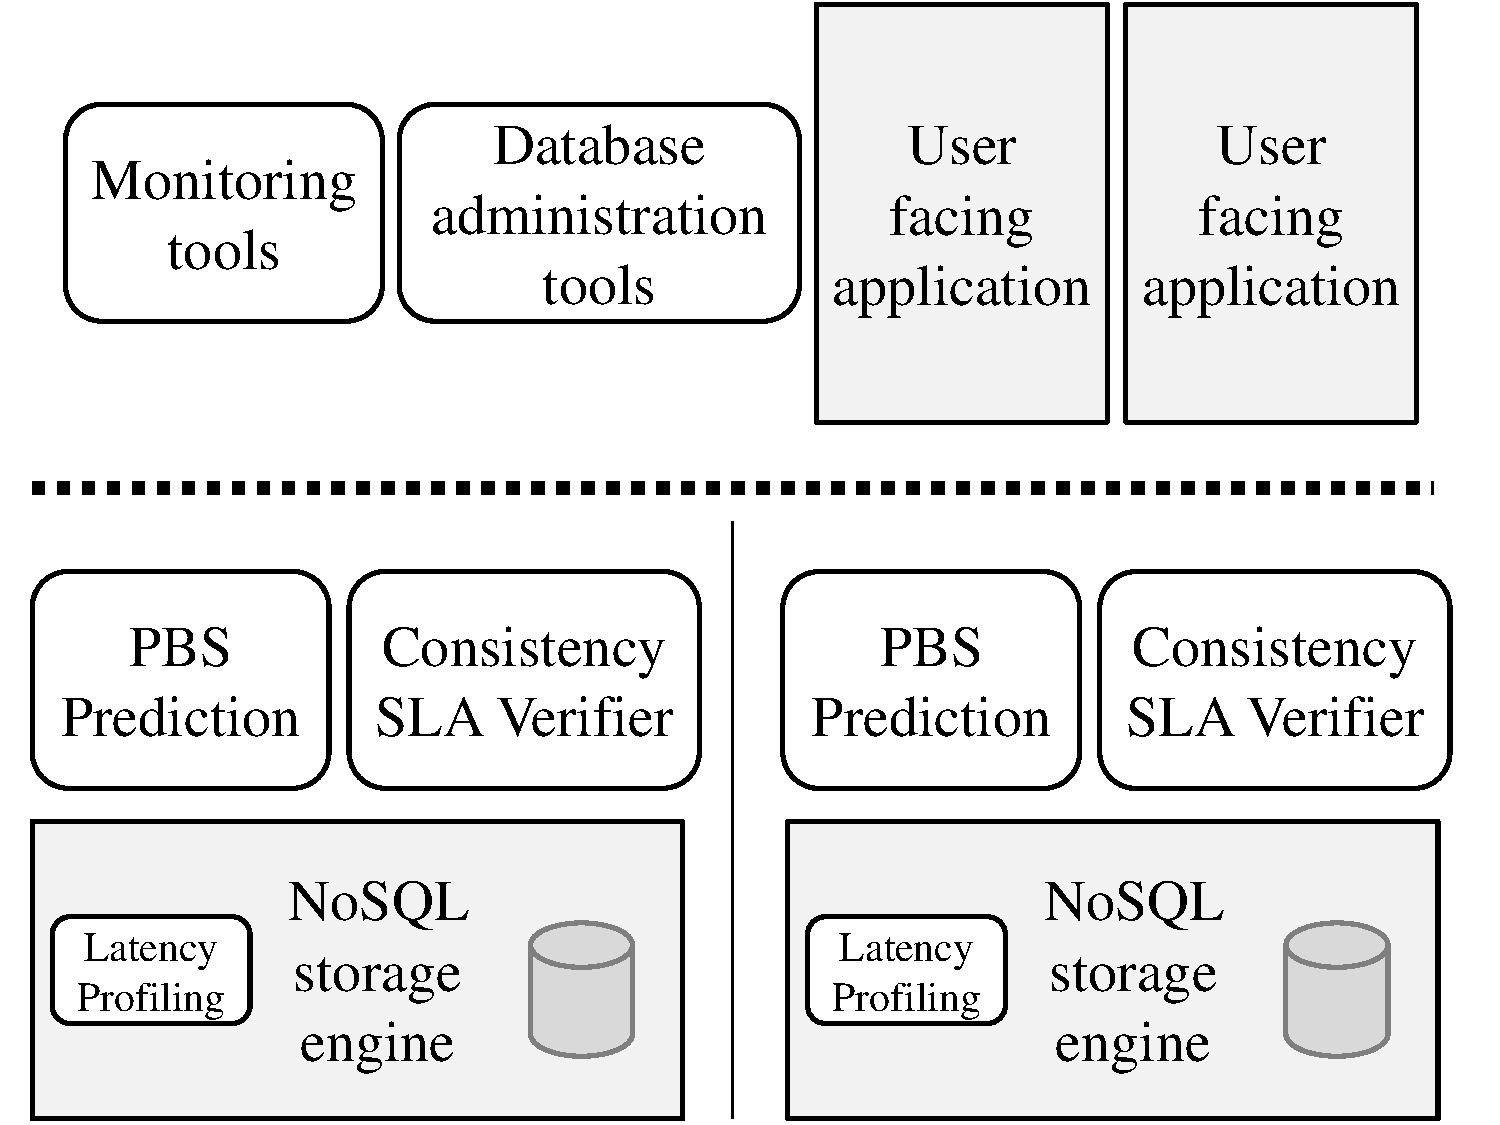
\includegraphics[width=.90\columnwidth]{figs/pbs-sys-arch.pdf}
\caption{Diagram showing how PBS metrics can be integrated into an existing
NoSQL datastore. The PBS prediction module and Consistency SLA verifier drive
the metrics used the monitoring framework.}
\label{fig:pbs-sys-arch}
\end{figure}

\subsection{Database Architecture}

The lower half of Figure~\ref{fig:pbs-sys-arch} shows the architecture changes
that are required to integrate PBS metrics into an existing distributed
database. In each storage node, we inject lightweight latency profiling and
introduce two new modules that help with consistency prediction and SLA
verification. These modules are designed to be a thin-layer on top of the
existing datastore and can be easily adapted to different systems.\\

%Walk through the system diagram - Explain what each component does. In
%particular explain how the latency collector feeds into the PBS prediciton
%module and how the Monte-Carlo simulation can be run using this data.
\textbf{PBS Prediction:} The PBS prediction module is responsible for
calculating the \textit{t-visibility} and
\textit{k-staleness}~\cite{pbs-vldb2012} for the
datastore. This latency profiling module is used to extract the latency for
writes, acks, reads and responses (WARS model) that are sent during replication.
This data is fed into the prediction module which keeps track of the most recent
latencies from all the operations.  Whenever a consistency prediction needs to
be made, these latencies values are used to perform a MonteCarlo simulation. We
execute a number of iterations of the simulation and estimate k-stateless,
t-visibility and the latency for the operations. In our Cassandra implementation
we found that the prediction finishes within a couple of seconds. \\ 


%Talk about how the simulation can be triggered by either the database
%administration tool or the Consistency SLA verifier module. The consistency sla
%verifier accepts SLA specifications from clients and periodically triggers the
%prediction module - This module also completes the loop and adjusts the value of
%N,R and W until the consistency SLA is met.

\textbf{Consistency SLA verifier:} One of the use cases of consistency
prediction is that the data store can use this data to provide SLAs on
consistency. This can be accomplished by a standalone module that tracks the
consistency and latency profile of queries over time. Database administrators
can specify the SLA required in terms of what is the maximum value of
t-visibility or k-staleness that is acceptable. The verification module
periodically triggers the PBS predictor. Based on the predictions, the values of
R and W are adjusted to ensure that the SLA is met while minimizing the latency
observed. Since the number of possible states is limited for small values of N,
our current implementation performs a complete search over the state space.
We have also formulated this as an integer linear program and are exploring if
we can use linear solver in the future.

\subsection{Userspace tools}
%Finally talk about how the database administration tool can also trigger the pbs
%prediction. Explain how this works with respect to nodetool and the flexibility
%they have with respect to the query inteface.
The PBS predictions are not only meant to be used by automated tools like the
SLA verifier but can also be used by database administrators to get more
insights into the latency-consistency trade-offs for their deployment. In our
Cassandra implementation, we have added a new command
\textit{predictconsistency} to \textit{nodetool}, a widely used administration
interface.  The \textit{predictconsistency} command allows a flexible interface
for performing PBS prediction. Database administrators can specify the
replication factor (N,R,W) to be used and the time at which a read is performed
after a write request. This allows administrators to perform what-if analysis
and project the impact on latency and consistency as their workload changes.
Finally, we also export the consistency metrics over a Java MBean interface,
meaning any tool that can handle MBean output can be used to display this
data.\\

%Last talk a little bit about the monitoring tools and how one can export the PBS
%metrics in a time series format and alert the users if some trigger has not been
%meet for the given time period.

In addition to automated consistency SLA verification, PBS can be used by administrators
to monitor the consistency their datastore is providing them. In contrast to
offline consistency verification schemes~\cite{podc-hp}, PBS predictions provide
a lightweight mechanism that can be used for monitoring. A monitoring tool like
Ganglia~\cite{massie2004ganglia} or DataStax's OpsCenter~\cite{datastax-opscenter} can be used to
issue  periodic PBS prediction requests and plot the values of t-visibility and
k-staleness as a timeseries. This can then be integrated with rule-based
alerting systems to page an operator if the value of t-visibility is beyond a
particular threshold for an extended time period.
